
\chapter{Technical Background}	\label{chap:background}
\section{General processing chain}
%audio - pre-processing - feat. extraction - machine learning
% unseen audio - pre-processing - feat. extraction  - run through model - result
\section{Audio features}
%mfcc, sdc, (rasta-)plp, trap; mention filterbank feats...?
%TODO: write intro
\subsection{Perceptive Linear Predictive features (PLPs)} 
PLP features, first introduced in \cite{hermansky90}, are among the most frequently used features in speech processing. They are based on the idea to use knowledge about human perception to emphasize important speech information in spectra while minimizing the differences between speakers. In this work, model orders of 13 and 36 are used. Deltas and double deltas between frames are also calculated. PLPs are tested with and without RASTA pre-processing \cite{rasta_plp}.
\subsection{Mel-Frequency Cepstral Coefficients (MFCCs)} 
%!
Just like PLPs, MFCCs are frequently used in all disciplines of automatic speech recognition \cite{zissman}. In this work, 13 or 20 coefficients were kept, depending on the experiment. Additionally, deltas and double deltas were calculated.
\subsection{Shifted Delta Cepstrum (SDCs)} 
Shifted Delta Cepstrum features were first described in \cite{bielefeld} and have since been successfully used for speaker verification and language identification tasks on pure speech data \cite{torres} \cite{campbell} \cite{allen}. They are calculated on MFCC vectors and take their temporal evolution into account. Their configuration is described by the four parameter $N-d-P-k$, where $N$ is the number of cepstral coefficients for each frame, $d$ is the time context (in frames) for the delta calculation, $k$ is the number of delta blocks to use, and $P$ is the shift between consecutive blocks. The delta cepstrals are then calculated as:
\begin{equation}
\Delta c(t) = c(t+iP+d)+c(t+iP-d), 0<=i<=k
\end{equation}
with $c \in [0, N-1]$ as the previously extracted cepstral coefficients. The resulting $k$ delta cepstrals for each frame are concatenated to form a single SDC vector of the length $kN$. We used the common parameter combination $N=7, d=1, P=3, k=7$.
\subsection{TempoRal Patterns (TRAP)} 
TRAPs were developed by Hermansky \cite{traps1} \cite{traps2} and have been used successfully in a number of speech recognition tasks. In contrast to MFCCs, which only consider a single spectral frame at a time, TRAPs take the spectral development over time into account. Spectral bands are calculated for a fixed time context around an audio frame. Each band's trajectory is then normalized, windowed, and decorrelated using a DCT. All the DCT coefficients for all bands are concatenated to a single feature vector for the center frame. These coefficients are then usually used to train Neural Networks for phoneme recognition \cite{yan_barnard}\cite{matejka} in order to form TRAP features.  However, in this work, the coefficient vector is used directly as a feature to train various models. Figure \ref{fig:traps} shows the extraction process. In this work, 8 linear spectral bands were extracted with a time context of 20 frames, and the first 8 DCT coefficients were kept.
\begin{figure}
 \centerline{\framebox{
 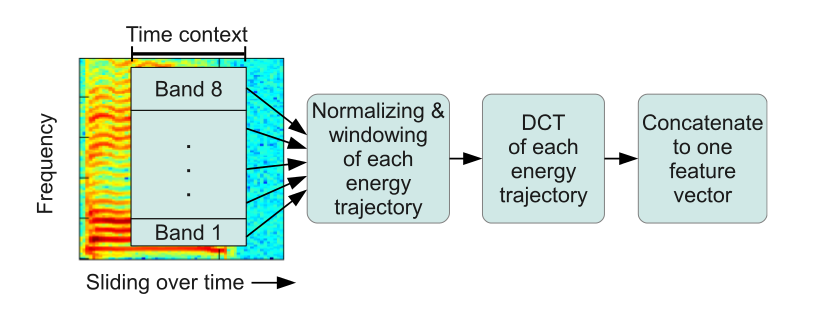
\includegraphics[width=\columnwidth]{images/trap_extraction.png}}}
 \caption{TRAP extraction process \cite{jens}}
 \label{fig:traps}
\end{figure}


\section{Recognition algorithms}
This section describes the various recognition algorithms employed throughout this thesis, most of which are Machine Learning methods. 
%DTW
Gaussian Mixture Models (GMMs), Hidden Markov Models (HMMs), and Support Vector Machines (SVMs) are three traditional approaches that are used as the basis of many new approaches, and were used for several starting experiments. i-Vector processing is a relatively new, more sophisticated approach that bundles several other machine learning techniques.\\
In recent years, Deep Learning has become the standard for machine learning applications \cite{}. This chapter also describes a new approach that was used extensively in this work: Deep Neural Networks (DNNs).

\subsection{Dynamic Time Warping}
%!
\subsection{Gaussian Mixture Models}
%256
%!
\subsection{Hidden Markov Models}
%!

\subsection{Support Vector Machines}
%! clean up
In all supervised classification tasks, a training data set and a classification data set are provided. Each of these sets consists of previously extracted features of the training entities (or musical pieces in the case of genre classification) and, for the training data set, annotation labels (or genres in the case of genre classification). The training data set is denoted here as pairs of $\left(\mathbf{x}_{i}, y_{i}\right), i=1..l$, with $\textbf{x}_i \in \mathbb{R}^{n}$ being the feature vectors and $y_{i}$ being their assigned classes. The classifier tries to find similarities behind the training data for each label and separation conditions between the labels. With this information, the classifier is then able to assign a label to the classification data entities.\\
SVMs attempt to solve this problem by grouping the training data vectors $\mathbf{x}_{i}$ and finding separating (hyper-)planes (with the normal vector $\mathbf{w}$ and the offset $b$) between the points of the different classes (or annotation labels) $y_{i}$. In doing so, they try to maximise the margin between the plane and the data points. Additionally, the feature vectors may be transformed into a higher-dimensional space by the function $\phi(\textbf{x}_i)$ to make them more easily separable (as demonstrated in figure \ref{fig:svm_transformation}).\newpage
In \cite{techreport:practical_svm}, this training process is expressed (for a two-class problem) as:
\begin{equation*}
\begin{aligned}
& \min\limits_{\mathbf{w},b,\xi} & & \frac{1}{2}\mathbf{w}^{T}\mathbf{w} + C \sum\limits_{i=1}^{l}\xi_{i} \\
& \text{subject to} & & y_{i}(\mathbf{w}^{T} \phi(\mathbf{x}_{i})+b) \geq 1-\xi_{i} , \\
&&& \xi_{i} \geq 0
\end{aligned}
\end{equation*}
(with $\xi_{i}$ being a slack variable and $C > 0$ being a penalty parameter for the error term, higher $C$s allowing for fewer outliers (\cite{article:intro_svm}).
\begin{figure}[htbp]
	\centering
	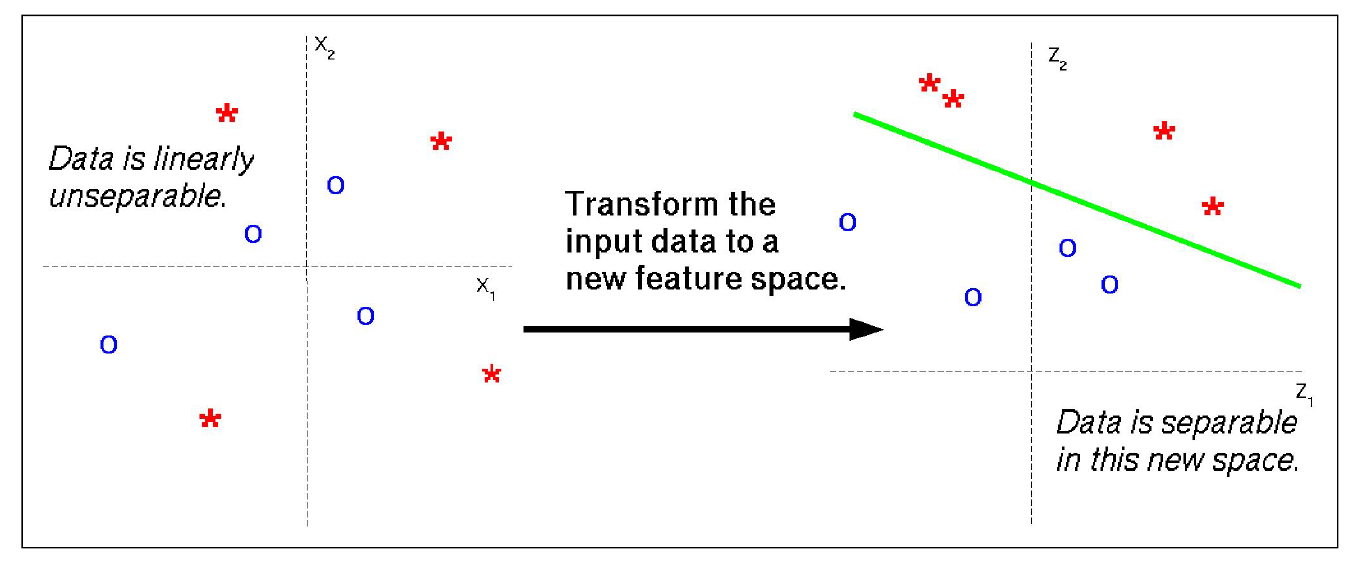
\includegraphics[width=0.9\textwidth]{images/svm_transformation.png}
	\caption{A set of data points which cannot be separated linearly in their original form (left), but can be separated after transformation into another space (right) \cite{article:intro_svm}}
	\label{fig:svm_transformation}
\end{figure}
\medskip
\\
$K(\mathbf{x}_{i},\mathbf{x}_{j}) \equiv \phi(\mathbf{x}_{i})^{T} \phi(\mathbf{x}_{j})$ is called the \textit{kernel function}. Several variants are possible, e.g. a linear one:
\begin{equation}
K(\mathbf{x}_{i},\mathbf{x}_{j}) = \mathbf{x}_{i}^{T}\mathbf{x}_{j}
\end{equation}
It is often useful to use a non-linear kernel because the data points may not be linearly separable (even after the transformation into a higher-dimensional space). An example is shown in figure \ref{fig:svm_kernels}. The RBF kernel (Radial Basis Function) is a popular one:
\begin{equation}
K(\mathbf{x}_{i},\mathbf{x}_{j}) = e^{-\gamma \parallel \mathbf{x}_{i} - \mathbf{x}_{j} \parallel^{2}}, \gamma > 0
\end{equation}
\begin{figure}[htbp]
	\centering
	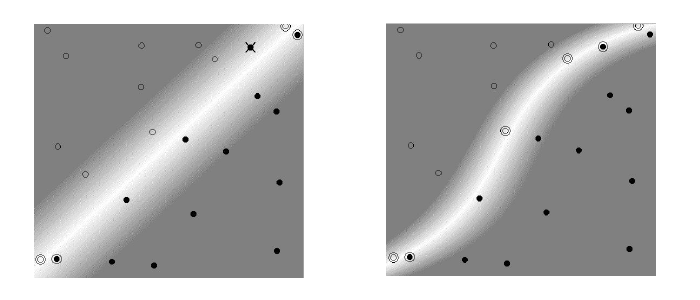
\includegraphics[width=0.9\textwidth]{images/svm_kernels.png}
	\caption{A set of data points which cannot be separated using a linear kernel (left), but can be separated with a polynomial kernel (right) \cite{article:svm_tutorial}}
	\label{fig:svm_kernels}
\end{figure}
\medskip
\\
As can be seen from the above equations, $C$ and $\gamma$ are free parameters. Their optimum values depend on the actual training data vectors. In \cite{techreport:practical_svm}, a grid search during each training is suggested to find them. 
\medskip
\\
The presented training process is appropriate for a two-class problem. For multi-class problems, one-vs-one trainings for all combinations of classes are performed. Then,all of the developed classifiers are used for the classification of the evaluation data and a voting strategy is applied to determine the resulting class. This procedure is not quite in agreement with the one used in the feature selection algorithm (IRMFSP, see section \ref{subsec:irmfsp}), as this algorithm selects features to separate all classes at once, rather than on a one-vs-one basis.


\subsection{i-Vector processing}
I-Vector (identity vector) extraction was first introduced in \cite{Dehak2011} and has since become a state-of-the-art technique for various speech processing tasks, such as speaker verification, speaker recognition, and language identification \cite{Martinez2011}. To our knowledge, it has not been used for any Music Information Retrieval tasks before. \\
The main idea behind i-vectors is that all training utterances contain some common trends, which effectively add irrelevance to the data in respect to training. Using i-vector extraction, this irrelevance can be filtered out, while only the unique parts of the data relevant to the task at hand remain. The dimensionality of the training data is massively reduced, which also makes the training less computationally expensive. As a side effect, all feature matrices are transformed to i-vectors of equal length, eliminating problems that are caused by varying utterance lengths.\\
Mathematically, this assumption can be expressed as:
\begin{equation}
M(u) = m+Tw
\end{equation}
In this equation, $M(u)$ is the GMM supervector for utterance $u$. The supervector approach was first presented in \cite{reynolds00} and has since been successfully applied to a number of speech recognition problems. A music example can be found in \cite{Charbuillet2011}. $m$ represents the language- and channel-independent component of $u$ and is estimated using a Universal Background Model (UBM). $T$ is a low-rank matrix modeling the relevant language- and channel-related variability, the so-called Total Variability Matrix. Finally, $w$ is a normally distributed latent variable vector: The i-vector for utterance $u$.

\paragraph*{Step 1: UBM training} A Universal Background Model (UBM) is trained using Gaussian Mixture Models (GMMs) from all utterances. This UBM models the characteristics that are common to all of them.
\paragraph*{Step 2: Statistics extraction} 0th and 1st order Baum-Welch statistics are calculated for each of the utterances from the UBM according to:
\begin{equation}
N_c(u)=\sum_{t=1}^{L} P(c|y_t,\Omega)
\end{equation}
\begin{equation}
\widetilde{F_c}(u)=\sum_{t=1}^{L} P(c|y_t,\Omega)(y_t-m_c)
\end{equation}
where $u={y_1,y_2,...,y_L}$ denotes an utterance with $L$ frames, $c=1,...,C$ denotes the index of the Gaussian component, $\Omega$ denotes the UBM,  $m_c$ is the mean of the UBM mixture component $c$, and $P(c|y_t,\Omega)$ denotes the posterior probability that the frame $y_t$ was generated by mixture component $c$. As the equation shows, the 1st order statistics are centered around the mean of each mixture component.\\
\paragraph*{Step 3: T matrix training}
Using the Baum-Welch statistics for all utterances, the Total Variability Matrix $T$ is now trained iteratively according to:
\begin{equation}\label{equ:trainT}
w = (I+T^t \Sigma^{-1} N (u) T)^{-1}T^t \Sigma^{-1} \widetilde{F}(u)
\end{equation}
using Expectation Maximization.
\paragraph*{Step 4: Actual i-vector extraction}
Finally, an i-vector $w$ can be extracted for each utterance using equation \ref{equ:trainT} again. This can also be done for unseen utterances, using a previously trained $T$.


\subsection{Artificial Neural Networks}
%!

\section{Evaluation}
\subsection{Evaluation of phoneme recognition and alignment tasks}
%alignment? - duration acc. - no, mean error
\subsection{Evaluation of language identification tasks}
\subsection{Evaluation of keyword spotting tasks}

\section{Speech recognition systems}
\subsection{Phoneme recognition}
\subsection{Forced alignment}
\subsection{Language identification}
Language identification has been extensively researched in the field of Automatic Speech Recognition since the 1980's. A number of successful algorithms have been developed over the years. An overview over the fundamental techniques is given by Zissman in \cite{zissman}.\\
Fundamentally, four properties of languages can be used to discriminate between them:
\begin{description}
	\item[Phonetics] The unique sounds that are used in a given language.
	\item[Phonotactics] The probabilities of certain phonemes and phoneme sequences.
	\item[Prosody] The ``melody'' of the spoken language.
	\item[Vocabulary] The possible words made up by the phonemes and the probabilities of certain combinations of words.
\end{description}
Even modern system mostly focus on phonetics and phonotactics as the distinguishing factors between languages. Vocabulary is sometimes exploited in the shape of language models.\\
Zissman mentions Parallel Phone Recognition followed by Language Modeling (PPRLM) as one of the basic techniques. It requires audio data, language annotations, and phoneme annotations for each utterance. In order to make use of vocabulary characteristics, full sentence annotations and word-to-phoneme dictionaries are also necessary.\\
Using the audio and phoneme data, acoustic models are trained. They describe the probabilities of certain sound and sound sequences occurring. This is done separately for each considered language. Similarly, language models are generated using the sentence annotations and the dictionary. These models describe the probabilities of certain words and phrases. Again, this is done for each language.\\
New audio examples are then run through all pairs of acoustic and language models, and the likelihoods produced by each model are retained. The highest acoustic likelihood, the highest language likelihood, or the highest combined likelihood are then considered to determine the language. This approach achieves up to $79\%$ accuracy for ten languages \cite{muthusamy}.\\
Another approach uses the idea to train Gaussian Mixture Models for each language. This technique can be considered a ``bag of frames'' approach, i.e. the single data frames are considered to be statistically independent of each other. The generated GMMs then describe probability densities for certain characteristics of each language. Using these, the language of new audio examples can be easily determined.\\
GMM approaches used to perform worse than their PPRLM counterparts, but the development of new features has made the difference negligible \cite{singer}. They are in general easier to implement since only audio examples and their language annotations are required. Allen et al. \cite{allen} report results of up to $76.4\%$ accuracy for ten languages. Different backend classifiers, such as Multi-Layer Perceptrons (MLPs) and Support Vector Machines (SVMs) \cite{campbell} have also been used successfully instead of GMMs.

\subsection{Keyword spotting}




